\myChapter{Testy}\label{ch:tests}
%************************************************

\section{Cele}

Głównym zadaniem przeprowadzonych testów było zbadanie zachowania stworzonego systemu i oprogramowania pod kątem wykorzystania w grach wideo\graffito{Wynika to ze studiowania na specjalności Technologii Gier i Symulacji Komputerowych.}. Nie jest jednak trudno sobie wyobrazić inne dziedziny, w których można wykorzystać system, jak np.:
\begin{itemize}
 \item medycyna \ppauza manipulacja trójwymiarowymi obrazami skanów pacjentów,
 \item cyfrowe modelowanie \ppauza szybkie prototypowanie modeli,
 \item tworzenie filmów \ppauza przechwytywanie ruchu.
\end{itemize}

Głównym atutem systemu w tych dziedzinach jest naturalny sposób manipulacji i~interakcji z komputerem ze względu na pobieranie dodatkowo \ppauza w odróżnieniu od standardowego zostawu klawiatura + myszka \ppauza trzeciego wymiaru.

\section{Metody}
Aby określić przydatność systemu, należy zbadać kilka czynników. Ich wagi będą różnić się, w zależności od planowanego wykorzystania, jednak można zauważyć, że należy dążyć do optymalizacji cech takich jak:
\begin{itemize}
 \item dokładność,
 \item stabilność,
 \item niezawodność,
 \item prostota użytkowania,
 \item kompatybliność z oprogramowaniem,
 \item szybkość.
\end{itemize}


\section{Wyniki}
% dokladnosc
\paragraph{Dokładność}
Dokładność systemu została już określona w sekcji \ref{section:precision}, pozwolę więc sobie jedynie przytoczyć obliczone parametry.

Istnieją dwa rodzaje ograniczeń: spowodowane stworzonym oprogramowaniem oraz spowodowane wykorzystanym sprzętem. Ominięcie tych pierwszych jest stosunkowo łatwe\graffito{Trzeba liczyć się z faktem, że można natknąć się na ograniczenia mikrokontrolera.} i~wymaga tylko zmiany pewnych parametrów oraz ponowne zaprogramowanie układu. W przypadku drugiego typu ograniczeń należy spodziewać się konieczności modyfikacji układu, jeśli chciałoby się zwiększać dokładność.

Mikrokontroler jest w stanie mierzyć pozycję markera z dokładnością do 0,34mm\graffito{Równania odpowiednio \ref{eq:microcontroller_limit} i \ref{eq:sound_limit}.}, natomiast wykorzystanie sygnałów ultradźwiękowych o częstotliowści 40kHz nakłada na system ograniczenie dokładności do 8,5mm, a zatem ograniczenie całego systemu wynosi 8,5mm.

Chociaż w wielu przypadkach taka dokładność jest zupełnie wystarczająca, pozostawia jednak trochę do życzenia.

% stabilnosc
\paragraph{Stabilność}
Pomimo przytoczonej powyżej, relatywnie małej, dokładności układ wykazuje pewną niestabilność, która objawia się drganiem odtworzonej pozycji markera. Widać to dobrze na rysunku \ref{fig:position_shaky}, którego górna część pokazuje odtworzoną pozycję w trzech wymiarach. Wszystkie dane, a w szczególności wartość $X$ oraz $Z$, wykazują kilkucentymetrowe drgania pomimo stabilnego umocowania zarówno układu jak i markera.

\begin{figure}
 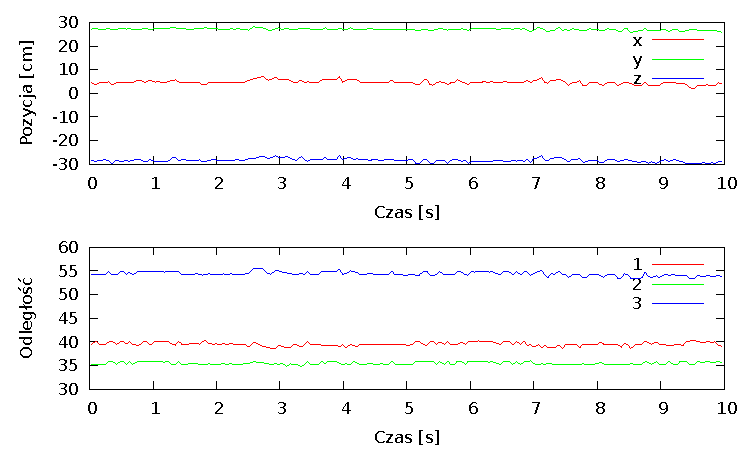
\includegraphics[width=\textwidth]{gfx/pozycja/pozycja.pdf}
 \caption[Wykres pozycji i odległości jednego z markerów]{Wykres pozycji i odległości od czujników jednego z~markerów w~stałej pozycji}
 \label{fig:position_shaky}
\end{figure}

% niezawodność
%\graffito{coś trzeba napisać o niezawodności}

% prostota użytkowania
\paragraph{Prostota użytkowania}
Starałem się zaprojektować system w taki sposób, aby korzystanie z niego było możliwie proste, jednak wymogi systemu powodują, że korzystanie z niego nie jest tak proste, jak ma to miejsce w przypadku systemów ,,konkurencyjnych'' \graffito{Wiimote, Sixaxis, Kinect...}.

Aby móc w pełni wykorzystać oprogramowanie, a~w~szczególności program \textsmaller{\nameref{sec:app_stickman}}, wymagane jest dokonanie \index{kalibracja}kalibracji. Nie jest to czynność trudna, lecz wymóg wykonania jej każdorazowo po uruchomieniu może zniechęcać użytkowników.

Kalibracja ma na celu ustawienie wewnętrznych parametrów programu, które będą pozwalały na dokładniejsze odwzorowanie ruchów użytkownika. Na wykorzystywane parametry składają się długość ręki, pozycja ramienia i rotacja ramienia.

W zależności od trybu kalibracji wymagane jest pobranie dwóch lub trzech punktów kontrolnych; w tym celu należy:
\begin{enumerate}
 \item jeśli została już dokonana kalibracja od uruchomienia programu, należy ją zresetować za pomocą stosownego przycisku,
 \item ustawić rękę (marker) w ustalonej pozycji względem ciała,
 \item nacisnąć przycisk informujący program o ustawieniu markera,
 \item powtórzyć czynność dla pozostałych punktów kontrolnych,
 \item gdy zostaną pobrane wszystkie punkty kontrolne, należy nacisnąć przycisk wyzwalający kalibrację, co spowoduje ustawienie trybu skalibrowanego.
\end{enumerate}

Wykonanie tej procedury spowoduje przekształcanie układu współrzędnych urządzenia na układ współrzędnych związany z użytkownikiem.

% kompatybilność z oprogramowaniem
\paragraph{Kompatybilność z oprogramowaniem}
Program wykorzystuje do komunikacji z komputerem protokół \index{RS232}\textsmaller{RS232}. Jest to standard komunikacji szeregowej niegdyś bardzo często dostępny w komputerach, jednak dziś odpowiednie złącza i interfejsy dostępne są za sprawą stosunkowo niedrogich adapterów wpinanych do portu \index{USB}\textsmaller{USB}.

Chociaż do uruchomienia komunikacji z wykorzystaniem modułu \index{USART}\textsmaller{USART}\graffito{\textsmaller{USART} \ppauza Universal Synchronous and Asynchronous serial Receiver and Transmitter.} mikrokontrolera nie jest wymagane stosowanie zewnętrznego oscylatora, to jego wykorzystanie zmniejsza ilość błędów, jakie mogą zachodzić podczas transmisji.

Ze względu na brak możliwości zakupu stosownego oscylatora, zdecydowałem się wykorzystać wbudowany w mikrokontroler zadajnik częstotliowści. W takiej konfiguracji, w przypadku transmisji danych z prędkością 9600bps\graffito{\index{bps}bps \ppauza baud per second; symbole na sekundę; w~przypadku RS232 1 symbol to 1 bit.} błąd wynosi zaledwie 0,2\%.\label{sec:usart_error}

Wynika to z równania określającego prędkość transmisji w mikrokontrolerze:
\begin{equation}
F_\textrm{USART} = \frac{F_\textrm{cpu}}{16 \cdot \textrm{(UBRR + 1)}}
\end{equation}
gdzie:
\begin{description}
  \item[$F_\textrm{USART}$] \ppauza~prędkość komunikacji w bps,
  \item[$F_\textrm{cpu}$] \ppauza~częstotliwość procesora,
  \item[UBRR] \ppauza~rejestr konfiguracji modułu \textsmaller{USART}.
\end{description}

Każda z tych wartości musi być liczbą całkowitą, co powoduje, że wykorzystując częstotliowść 8MHz nie jest możliwym uzyskanie dokładnych prędkości, jakie obsługiwane są przez pozostałe urządzenia wykorzystujące ten protokół, lecz wartości bardzo do nich zbilżone.

% str 136

Moje doświadczenie z mikrokontrolerami pokazuje, że wartość ta jest dostatecznie mała, aby można było założyć, że trasmisja jest dokładna.

Wykorzystany do komunikacji interfejs oraz zaproponowany protokół\graffito{Protokół opisano w~sekcji \ref{sec:protocol}.} jest bardzo prosty, co pozwala na dodanie obsługi systemu do dowolnego programu pragnącego skorzystać z tej możliwości znikomym nakładem pracy.

Stanowiłoby to duży atut systemu w przypadku jego popularyzacji.

\paragraph{Szybkość}
Niestety, szybkość układu pozostawia wiele do życzenia.

Istnieje kilka czynników, które można podejrzewać o spowalnianie działania. Rozpatrzmy po kolei każdy z nich.
\newline
\newline
\textsl{Wydajność obliczeń}\graffito{Obliczenia dotyczą głównie przekształcania układu współrzędnych.}
Aby nie obciążać zbędną pracą mikrokontrolera, który na dodatek nie posiada wystarczającej mocy obliczeniowej, obliczenia dokonywane są dopiero na komputerze\graffito{Jeśli dana aplikacja faktycznie takich obliczeń wymaga.}. Chociaż w celu pełnego przywrócenia układu współrzędnych użytkownika z dowolnego ustawienia odbiorników wymaganych jest kilka obrotów oraz translacji punktów\graffito{Obrót i translacja wymagają mnożenia macierzy 4\texttimes 4 przez trójwymiarowy wektor.}, a także obliczanie wartości odwrotnych funkcji trygonometrycznych oraz normalizacje trójwymiarowych wektorów, to wykorzystanie procesora przez aplikację zarówno na laptopie wyposażonym w procesor \textsmaller{Intel Core 2 Duo T7700 2,40GHz} oraz komputerze stacjonarnym z procesorerm \textsmaller{Intel Core 2 Duo E6420 2,13GHz} jest znikome.

Przeprowadzone testy pokazują, że wspomniany powyżej laptop wykonuje 100000 pełnych cykli takich obliczeń w przeciągu 448ms, co oznacza, że jeden cykl obliczeń zajmuje niecałe 5\textmu s.
\newline
\newline
\textsl{Szybkość transmisji danych}
Szybkość transmisji danych zależy głównie od ilości danych przesyłanych protokołem określonym w sekcji \ref{sec:protocol} oraz prędkości tego protokołu.

W związku z błędami omówionymi w paragrafie \nameref{sec:usart_error}, możliwe są dwie prędkości, w których stopień błędu wynosi 2\textperthousand:
\begin{itemize}
 \item 9600bps
 \item 38400bps
\end{itemize}

Czas przesłania jednego raportu obliczamy wzorem:
\begin{equation}
 t = \frac{c \cdot r}{s} \cdot 1000
\end{equation}
gdzie:
\begin{description}
 \item[$t$] \ppauza~czas potrzebny na przesłanie raportu liczony w milisekundach,
 \item[$c$] \ppauza~ilość bitów w ramce, dla wykorzystanego trybu standardu \index{RS232}RS232 jest to wartość stała $c = 10$,
 \item[$r$] \ppauza~ilość bajtów w raporcie, dla zaprojektowanego protokołu jest to wartość stała $r = 8$,
 \item[$s$] \ppauza~wybrana szybkość.
\end{description}

Wykorzystując wymienione powyżej prędkości otrzymujemy czasy odpowiednio 8,3ms oraz 2,1ms.
\newline
\newline
\textsl{Szybkość pobierania danych}
Szybkość pobierania danych uzależniona jest od wykorzystanego zjawiska fizycznego i parametrów elementów je realizujących. W tym przypadku jest to zestaw nadajnik i odbiornik ultradźwiękowe wykorzystujące częstotliowść 40kHz. Związane z tym konsekwencje opisałem już częściowo w sekcji \ref{section:sound_limit}.

Należy zauważyć, że opisane wcześniej parametry tyczą się tylko pojedynczego okresu fali, nie jest natomiast zbadany czas w jakim dźwięk faktycznie dotrze z markera do odbiorników.

Przyjmując długość ręki 70cm\graffito{Długość ręki można zbadać za pomocą stworzonego systemu, moja ręka ma przeciętnie długość 68cm.} i wykorzystując przekstałcony wzór \ref{eq:sound_distance} uzyskujemy:
\begin{equation}
 t = \frac{x}{v} = \frac{70\textrm{cm}}{340\frac{\textrm{m}}{\textrm{s}}} = 0,7\textrm{m} \cdot \frac{1}{340}\frac{s}{m} \approx 0,002\textrm{s} = 2\textrm{ms}
 \label{eq:reporting_speed}
\end{equation}

Aby zagwarantować dotarcie sygnału markera do każdego z odbiorników, stworzone oprogramowanie nadaje go dopóty, dopóki nie zostanie odebrane potwierdzenie dotarcia z każdego z odbiorników. W powiązaniu z faktem, że nie można rozpocząć nadawania z innego markera, póki ,,kanał'' nie jest wolny, oznacza to, że sygnał z markera nadawany jest przynajmniej tak długo, jak długo zajmuje mu dotarcie do ostatniego z odbiorników.

W przyszłej wersji systemu można pokusić się o implementację metody, która niwelowałaby ten efekt. Działanie tej metody powinno wyglądać następująco:
\begin{enumerate}
 \item wysłać krótki sygnał z markera, o ustalonej z góry długości,
 \item jeśli nie zostanie uzyskane potwierdzenie otrzymania sygnału od wszystkich odbiorników w spodziewanym czasie (również odgórnie ustalonym), wysyłać sygnał z tego markera aż do uzyskania potwierdzenia ze wszystkich odbiorników.
\end{enumerate}
Chociaż metoda ta może wprowadzać pewne opóźnienia związane z oczekiwaniem na wygaszenie pinów odbiorników, to można przyjąć (jak pokazują testy), że większa część nadawanych sygnałów trafia do odbiorników, zatem skumulowana wydajność metody powinna być wyższa.
\newline
\newline
\textsl{Odbicia sygnału}
Kolejnym bardzo niekorzystnym dla systemu zjawiskiem są odbicia sygnału dźwiękowego od otoczenia. Podczas pierwszych testów urządzenia zauważyłem, że większa część pomiarów nijak ma się do rzeczywistości. Wykorzystując analizator logiczny zbadałem jakie faktycznie sygnały otrzymuje mikrokontroler na pinach odbiorników.

Rezultaty tego badania przedstawia rysunek \ref{fig:logic_analyzer}. Przedstawione są tam 4 wykresy, pierwszy ukazujący sygnał wyzwalający nadawanie, natomiast trzy pozostałe wykresy ukazują stan linii odbiorników w czasie. Z pierwszego wykresu łatwo odczytać, że zawarte są dwie próbki.

\begin{figure}
 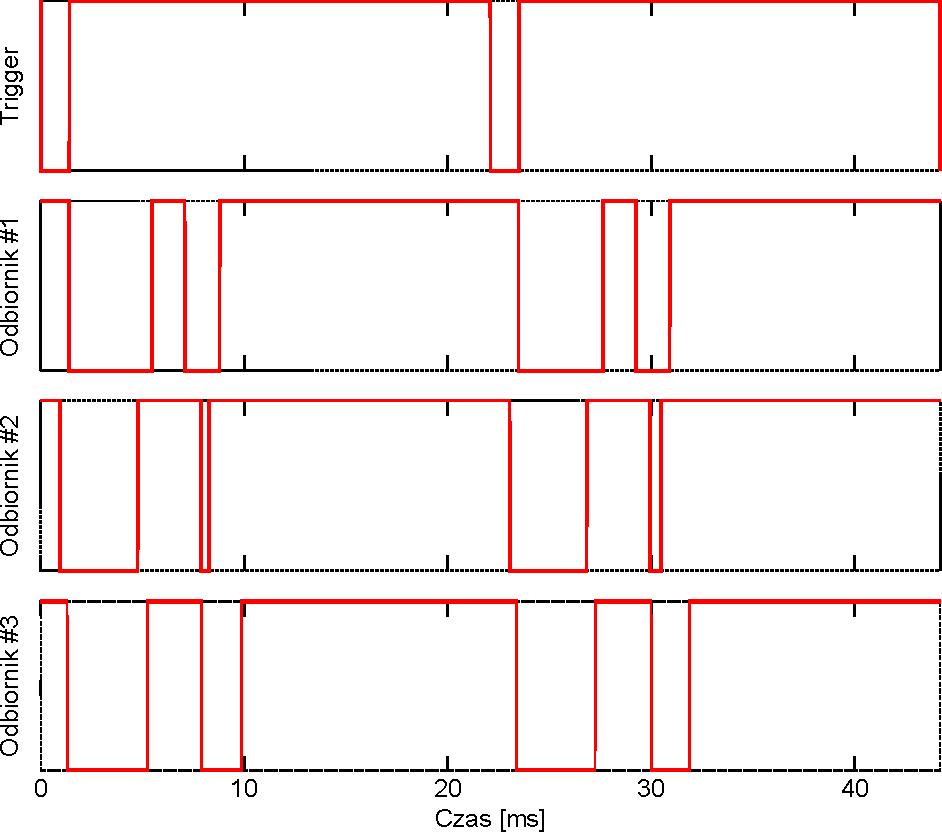
\includegraphics[width=\textwidth]{gfx/odbicia.pdf}
 \caption{Odbicia sygnału dźwiękowego}
 \label{fig:logic_analyzer}
\end{figure}

Porównując długość okresu, w którym nadawany jest sygnał (linia \texttt{Trigger} w stanie niskim) z długością okresu, kiedy odbiornik sygnalizuje odbieranie sygnału (linia odbiornika w stanie niskim), można dostrzec, że nie są one równe. Założyłem, że dźwięk \index{odbicia sygnału}odbił się od pobliskich elementów i dobiegł do odbiornika zanim nastąpił zanik sygnału bezpośredniego.

Na wykresie widać ponadto, że występuje ponowne wygaszenie linii po kilku milisekundach od zakończenia odbierania sygnału. W tym przypadku również zakładałem, że jest to sygnał odbity, który dobiegł do odbiornika.

Dokładniejsze badanie z wykorzystaniem oscyloskopu potwierdzają przypuszczenia. Wyniki tego badania prezentuje rysunek \ref{fig:oscilloscope}\graffito{Sygnał pomiędzy pinem mikrokontrolera, a~punktem testowym jest negowany.}.

\begin{figure}
 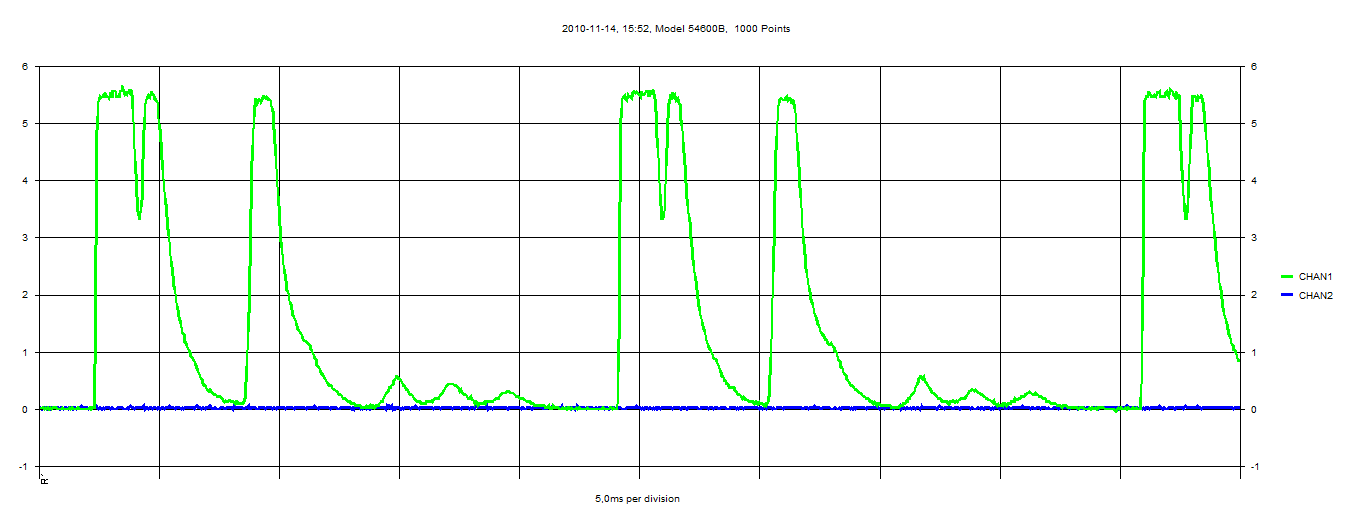
\includegraphics[width=\textwidth]{gfx/oscyloskop_1.png}
 \caption[Oscylogram sygnału w punkcie testowym]{Oscylogram sygnału w jednym z punktów testowych ukazujący odbicia sygnału}
 \label{fig:oscilloscope}
\end{figure}

\begin{figure}
 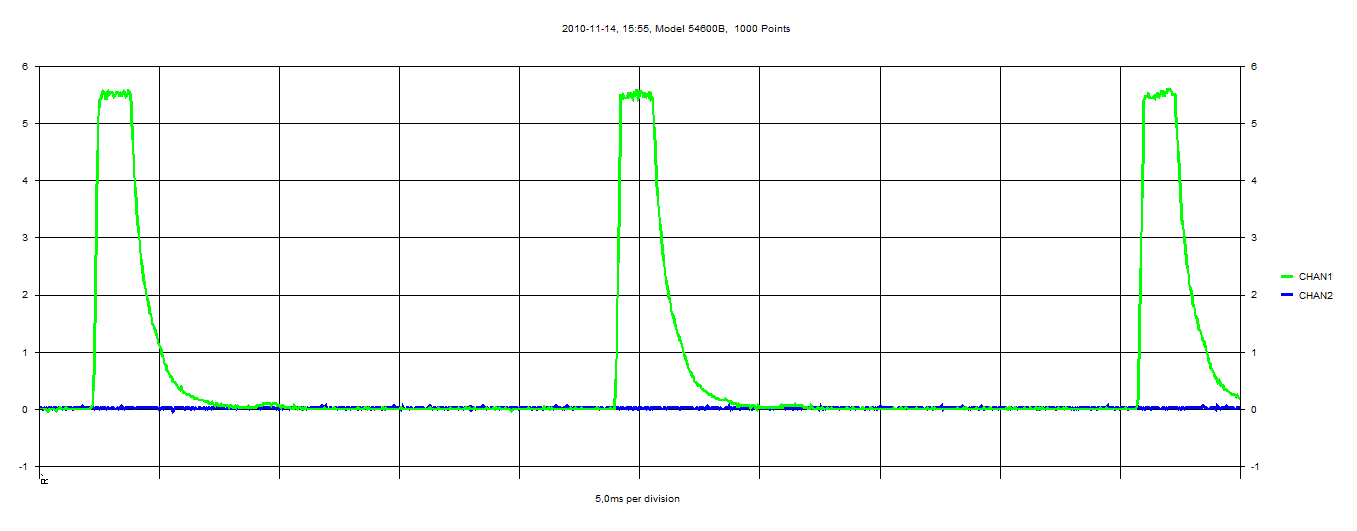
\includegraphics[width=\textwidth]{gfx/oscyloskop_attenuated.png}
 \caption{Oscylogram sygnału z dodatkowym tłumieniem}
 \label{fig:oscilloscope_attenuated}
\end{figure}


Aby uwolnić się od wspomnianej usterki, wprowadziłem do kodu mikrokontrolera wymuszone oczekiwanie, którego zadaniem jest upewnienie się, że wszystkie możliwe odbicia sygnału zaniknęły.

Wprawdzie ,,rozwiązanie'' działa, jednak znacząco spowalnia system \ppauza odstęp pomiędzy próbkami wynosi ponad 20ms.

Inną metodą obejścia tego problemu jest zwiększenie tłumienia sygnału rejestrowanego przez odbiornik. Praktyka pokazuje, że takie działanie faktycznie eliminuje problem, z drugiej jednak strony stanowczo pogarsza sprawność systemu, gdyż wymagane jest wtedy znacznie precyzyjniejsze celowanie markerem w odbiorniki. Oscylogram tego badania przedstawia rysunek \ref{fig:oscilloscope_attenuated}.

Z tego też powodu uznałem to za rozwiązanie gorsze, gdyż gracz, który jest docelowym użytkownikiem, w ferworze gry nie może pozwolić sobie na troskanie się sprawnością wykorzystywanego kontrolera.
\newline
\newline
\textsl{Podsumowanie szybkości działania}
Opierając się na wspomnianych powyżej testach widać, że czynnikiem powodującym największe opóźnienia jest dokładnie ten sam, który najtrudniej wyeliminować, czyli odbicia dźwięku. W związku z wprowadzonymi obejściami problemów, wydajność systemu ograniczona jest do najwyżej 25Hz\graffito{Pełen status nadawany jest co minimum 40ms.}.

\paragraph{Porównanie z innymi systemami}
Ze względu na możliwość dostępu do kontrolerów \index{Nintendo!Wiimote}\textsl{Wiimote} oraz \index{Sony!Sixaxis}\textsl{Sixaxis} postanowiłem przeprowadzić porównanie tych urządzeń z moim rozwiązaniem.
\newline

\textsl{Sixaxis}. W celu wyznaczenia prędkości raportowania statusu tego kontrolera wykorzystałem możliwość podłączenia go poprzez port \index{USB}USB oraz obsługę w systemie \index{Linux}Linux w wersji 2.6.35\graffito{Obsługa kontrolera dostępna jest od wersji 2.6.21 z 25.04.2007\citep{Br10}.}. Znając wielkość raportu, która wynosi 50 bajtów \citep{Br10}, wystarczy zbadać, jak prędko dane pojawiają się na urządzeniu przyporządkowanym kontrolerowi. 

Należy najpierw zbadać, do jakiego pliku został przyporządkowany do podłączonego urządzenia \ppauza należy w tym celu sprawdzić log kernela za pomocą polecenia \texttt{dmesg}, a następnie zbadać czas, w jakim odczytana zostanie określona z góry ilość danych. Eksperyment ten prezentuje listing~\ref{lst:sixaxis}.

\begin{listing}
  \lstinputlisting{listings/sixaxis.txt}
  \caption{Badanie prędkości kontrolera Sixaxis}
  \label{lst:sixaxis}
\end{listing}

W celu zbadania prędkości pojawiania się danych wykorzystałem program \texttt{dd} z argumentami:
\begin{description}
 \item[\texttt{if=/dev/hidraw4}] określa plik wejściowy, jest on odczytany z wyjścia programu \texttt{dmesg},
 \item[\texttt{of=/dev/null}] określa plik wyjściowy; przekierowując dane do pliku \texttt{/dev/null} upewniam się, że nie wystąpi ograniczenie prędkości operacją zapisu na dysku,
 \item[\texttt{bs=50}] określa rozmiar bloku danych, dzięki temu ustawiony jest bufor będący w stanie przyjąć cały pakiet danych, przez co unikane jest opóźnienie związane z alokacją pamięci,
 \item[\texttt{count=5000}] informuje program o ilości bloków, jakie mają zostać pobrane; ustaliłem dużą wartość w celu wyeliminowania opóźnień, jakie mogłyby wyniknąć w związku z inicjacją i zakończeniem transmisji.
\end{description}

Jak widać, w ciągu prawie dokładnie 50s przetransmitowanych zostało dokładnie 250000 bajtów. Wynika stąd, że prędkość raportowania wynosi
\begin{equation}
 \frac{250000\textrm{b}}{50\textrm{s}} : 50\frac{\textrm{b}}{\textrm{raport}} = 100\textrm{Hz}
\end{equation}

Analizując strukturę raportu, łatwo rozpoznać przyporządkowanie danych do przycisków i policzyć ilość przycisków ,,analogowych''\graffito{Przyciskami analogowymi zwykło nazywać się przyciski, które raportują jak bardzo są naciśnięte.}.
\newline

\index{Nintendo!Wiimote}\textsl{Wiimote}. W celu zbadania tego kontrolera wykorzystałem otwartoźródłową bibliotekę \texttt{CWiid}\citep{CWiid}. Zmodyfikowałem źródło jednego z programów, aby raportował czas przyjścia raportu, a następnie w oparciu o informacje o rozmiarach raportów (\citep{Wiibrew}) wybrałem raport, którego rozmiar wynosi dokładnie 18 bajtów, po czym obliczyłem ile raportów przyszło w danym okresie czasu.

Wyniki tego testu pokazuje listing~\ref{lst:wiimote}.

\begin{listing}
  \lstinputlisting{listings/wiimote.txt}
  \caption{Badanie prędkości kontrolera Wiimote}
  \label{lst:wiimote}
\end{listing}

Do pliku \texttt{log} zapisane zostały czasy w formacie \textit{sekundy.nanosekundy}\graffito{W systemach Linux czas reprezentowany jest jako ilość sekund od 1970-01-01T00:00:00Z (ISO 8601).}. W każdej linii pliku zapisana jest dokładnie jedna próbka, dlatego też ilość pobranych próbek wynosi 2500, co pokazuje program \texttt{wc} z argumentem \texttt{-l}. Różnicę pomiędzy rozpoczęciem, a zakończeniem rejestrowania danych prezentuje wynik działania programu \texttt{bc}. Wynika stąd, że prędkość raportowania wynosi
\begin{equation}
 \frac{2500}{25,45\textrm{s}} \approx 100\textrm{Hz}
\end{equation}

Porównanie tych i pozostałych parametrów kontrolerów prezentuje tabela \ref{tab:comparison}.


% http://texblog.net/latex-archive/layout/centering-figure-table/
\begin{table}[b]
  \myfloatalign
\noindent\makebox[\textwidth]{%
\index{Bluetooth} \index{USB} \index{RS232} \index{akceleromter} \index{żyroskop}
\begin{tabularx}{1.5\textwidth}{X|XXX} \toprule
    & \emph{Sixaxis} & \emph{Wiimote} & \emph{Nietoperz} \\ \hline
    Ilość przycisków & 17 & 11 & 0 \\
    Ilość przycisków ,,analogowych'' & 12 (nie licząc gałek) & 0 & 0 \\
    Komunikacja & Bluetooth, USB & Bluetooth & RS232 \\
    Prędkość raportowania & 100Hz & do 100Hz & poniżej 25Hz \\
    Wielkość raportu statusu & 50 bajtów & do 18 bajtów & 16 bajtów \\
    Możliwość dołączania rozszerzeń & \texttimes & \checkmark & \texttimes \\
    Detekcja ruchów & akcelerometr (3D), żyroskop (1D) & akcelerometr (3D) & ultradźwięki \\
    Dodatkowe funkcjonalności & zdalne uruchamianie konsoli, 4 diody, 2 gałki analogowe & zdalne uruchamianie konsoli, głośnik, kamera IR, 4 diody & 8 diod
  \end{tabularx}}
  \caption{Zestawienie funkcjonalności kontrolerów gier}
  \label{tab:comparison}
\end{table}